\begin{frame}
\titlepage
\end{frame}

\begin{frame}
	\frametitle{第 0 讲、课程简介}
	\linespread{1.5}
	\begin{enumerate}
	    \item 课程背景与主要内容
	    \item 资料与工具
	    \item 学习方法与要求
	\end{enumerate}
\end{frame}

\begin{frame}{高等数学}
	\linespread{1.2}\pause 
	\begin{block}{微积分(Calculus)}\pause 
		\begin{enumerate}
		  \item {\bf Wikipedia}\pause 
		\begin{itemize}
		  \item Latin, {\it a small stone used for counting} \pause 
		  \item {\it a branch of mathematics focused on {\b limits, functions,
		  	derivatives, integrals,}  and {\b infinite series}} \pause
	  	  \item {\it widespread application in {\b science, economics,} and {\b
	  	  engineering}} \pause
% 		  \item {\it constitues a major part of modern mathematics}\pause 
		\end{itemize}
		\item {\bf John von Neumann} ({\small\it The Mathematician, 1947})\pause
		\begin{itemize}
		  \item \alert{\it The calculus was the first achievement of modern
		  mathematics, and it is difficult to overestimate its importance.}
		\end{itemize}
% 		  \item James Stewart, Calculus(5th eds.), 2004\pause 
% 		  \begin{itemize}
% 		    \item {\it Calculus is fundamentally different from the mathematics that
% 		    you have studied previously}\pause 
% 		    \item {\it Calculus is less static and more {\b dynamic}}\pause 
% 		    \item {\it It is concerned with change and {\b motion}}\pause 
% 		    \item {\it It deals with quantities that {\b approach} other quantities}
% 		  \end{itemize}
		\end{enumerate}
	\end{block}
\end{frame}

\begin{frame}{课程内容}
	\linespread{1.5}\pause 
	\begin{center}
		\scalebox{0.275}{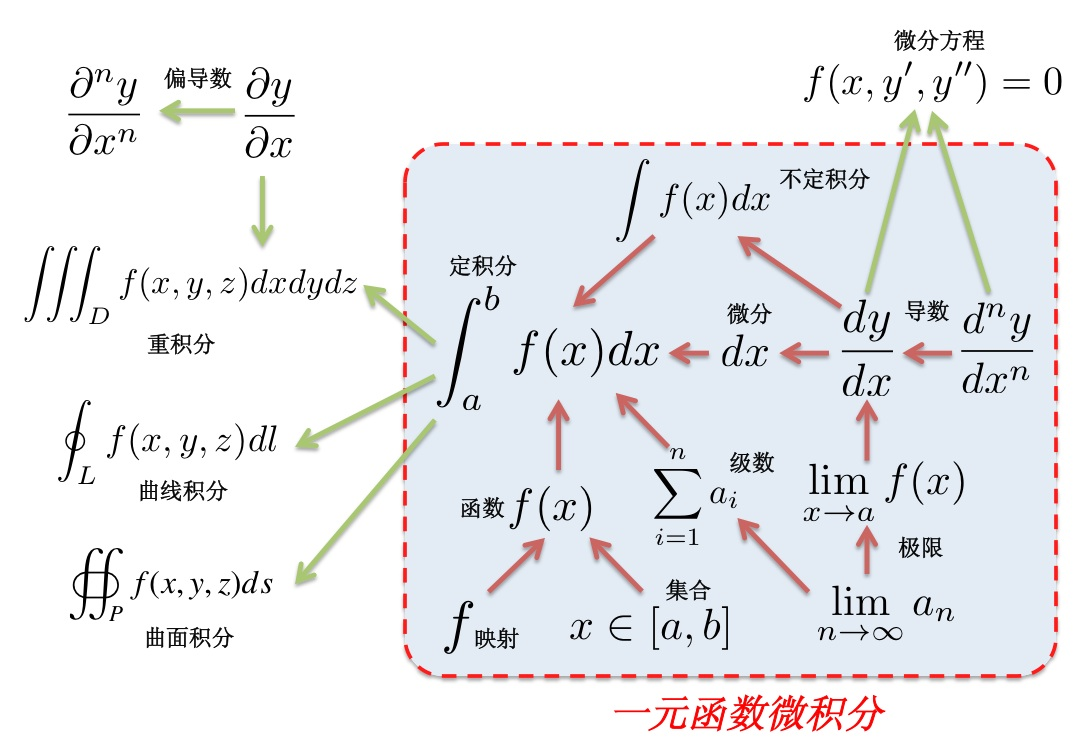
\includegraphics{./images/ch1/AM_architecture.jpg}}
	\end{center}
\end{frame}

\begin{frame}{参考资料}
	\linespread{1.3}\pause 
	\begin{enumerate}
	  \item {\bf 课程配套辅导}
	  \begin{itemize}
	    \item \alert{李建平 等,高等数学典型例题与解法(上、下),国防科技大学出版社,2009,长沙}\pause 
	  \end{itemize}
	  \item {\bf 参考书}\pause 
	  \begin{itemize}
	    \item {\b 同济大学数学系,高等数学(第六版,上、下),高等教育出版社,2006,北京}\pause 
	    \item 菲赫金哥尔茨,微积分学教程(第一至三卷),第8版,高等教育出版社,2006,北京\pause 
	    \item James Stewart, Calculus(5th eds.)(影印版,上、下册),高等教育出版社,2004,北京\pause
	  \end{itemize}
% 	  \item 任何有关教学内容和{\b 数学历史}的书籍
	\end{enumerate}
\end{frame} 

\begin{frame}[<+->]{学习方法}
	\linespread{1.4}
	\begin{enumerate}
	  \item {\bf 听课}\dotfill {\bb 30\%}
	  \begin{itemize}
	    \item 典型问题、典型方法
	    \item 师傅领进门,修行在个人
	  \end{itemize}
	  \item {\bf 练习}\dotfill {\bb 50\%}
	  \begin{itemize}
	    \item 熟能生巧!
	    \item 记忆!琢磨!
	  \end{itemize}
	  \item {\bf 思考}\dotfill {\bb 20\%}
	  \begin{itemize}
	    \item 总结!
	    \item 质疑!
	  \end{itemize}
	\end{enumerate}
\end{frame}

\begin{frame}[<+->]{要求}
	\linespread{1.4}
	\begin{enumerate}
	  \item {\bf 作业}
	  \begin{itemize}
	    \item 正确、规范、工整
	    \item no copy !!!!
	    \item 订正每一个错误!
	  \end{itemize}
	  \item {\bf 答疑}
	  \begin{itemize}
	    \item 有问必答
	    \item 除了问考试、问隐私
	  \end{itemize}
	\end{enumerate}
\end{frame}

\begin{frame}[<+->]{课堂}
	\linespread{1.2}
	\begin{columns}
		\column{0.4\textwidth}
		\begin{enumerate}
		  \item {\bf 安静!}
		  \item {\bf 安静!!}
		  \item {\bf 安静!!!}\\
		  \vspace{2em}
		  \pause
		  \alert{No to}
		  \begin{itemize}
		    \item Chatting
		    \item zZZ\ldots
		    \item anything noisy
		    \item \ldots
		  \end{itemize}
		\end{enumerate}
		\column{.6\textwidth}
		\pause
		\alert{Yes to}
		  \begin{itemize}
		    \item listen to me
		    \item discuss with me
		    \item do sth. you like \alert{quietly}
		    \item zzz\ldots
		    \item leave/enter the classroom \alert{quietly}
		    \item \ldots
		  \end{itemize}
	\end{columns}
\end{frame}

% \begin{frame}{Welcome}
% 	\linespread{1.3}\pause
% 	\begin{block}{George Polya}\pause
% 	{\it
% 		“A great discovery solves great problem \pause but there is a grain of
% 		discovery in ther solution of any problem. \pause Your problem may be
% 		modest; \pause but if it challenges your {\b curiosity} \pause and brings
% 		into play your inventive facilities, \pause and if you {\b solve it by your
% 		own means}, \pause you may experience the {\b tension} \pause and enjoy the
% 		{\b triumph} of discovery.”}
% 	\end{block}
% \end{frame}

\begin{frame}
	\linespread{1}
	\begin{center}
		\resizebox{8cm}{!}{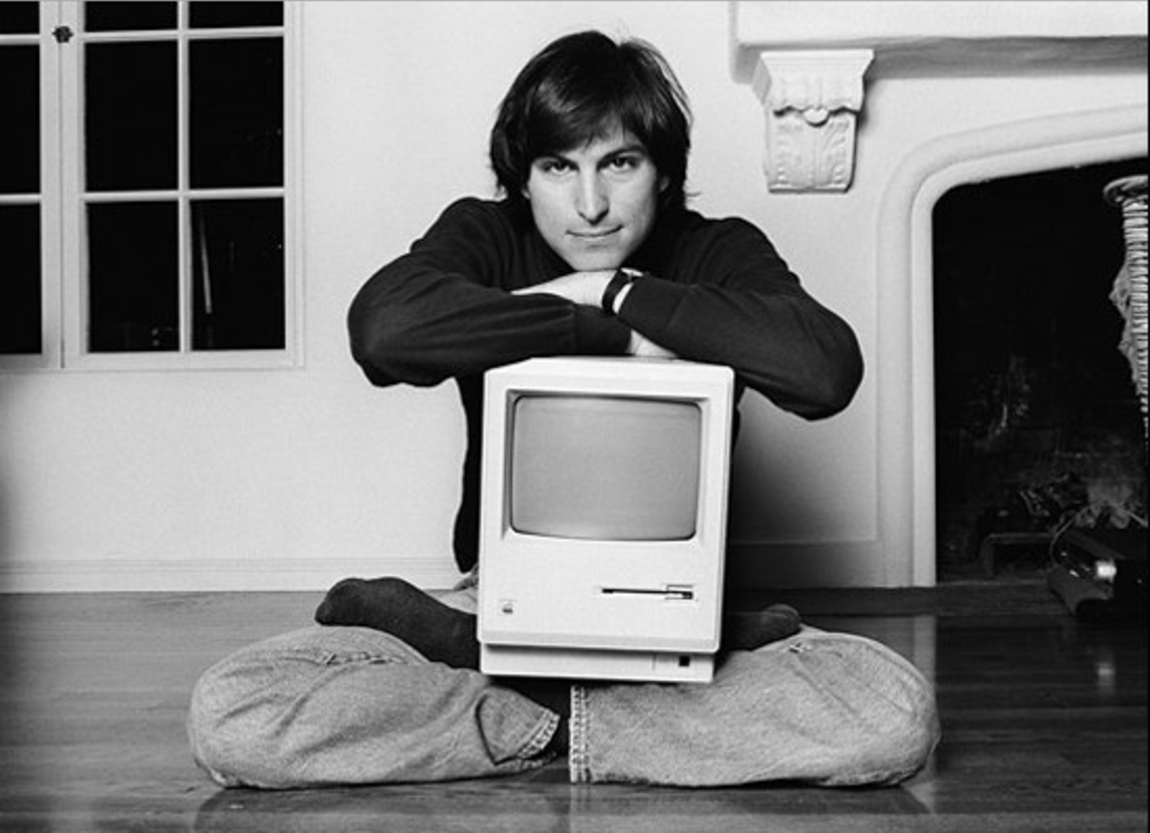
\includegraphics{./images/ch1/Jobs_Young.pdf}}\pause

		\bigskip
		{
% 			\fontspec{Myriad Pro}
			{\large Steve Jobs}

			{\footnotesize 1955-2011}
		}
	\end{center}
\end{frame}

\begin{frame}
	\linespread{1.2}
	\begin{center}
		{
% 		\fontspec{Myriad Pro}
		\small
			\ldots 1982\ldots 1997\ldots 1999\ldots 2002\ldots 2005\ldots 2007\ldots
			2010\ldots 2011 \ldots}
		\bigskip\pause

		\resizebox{!}{7cm}{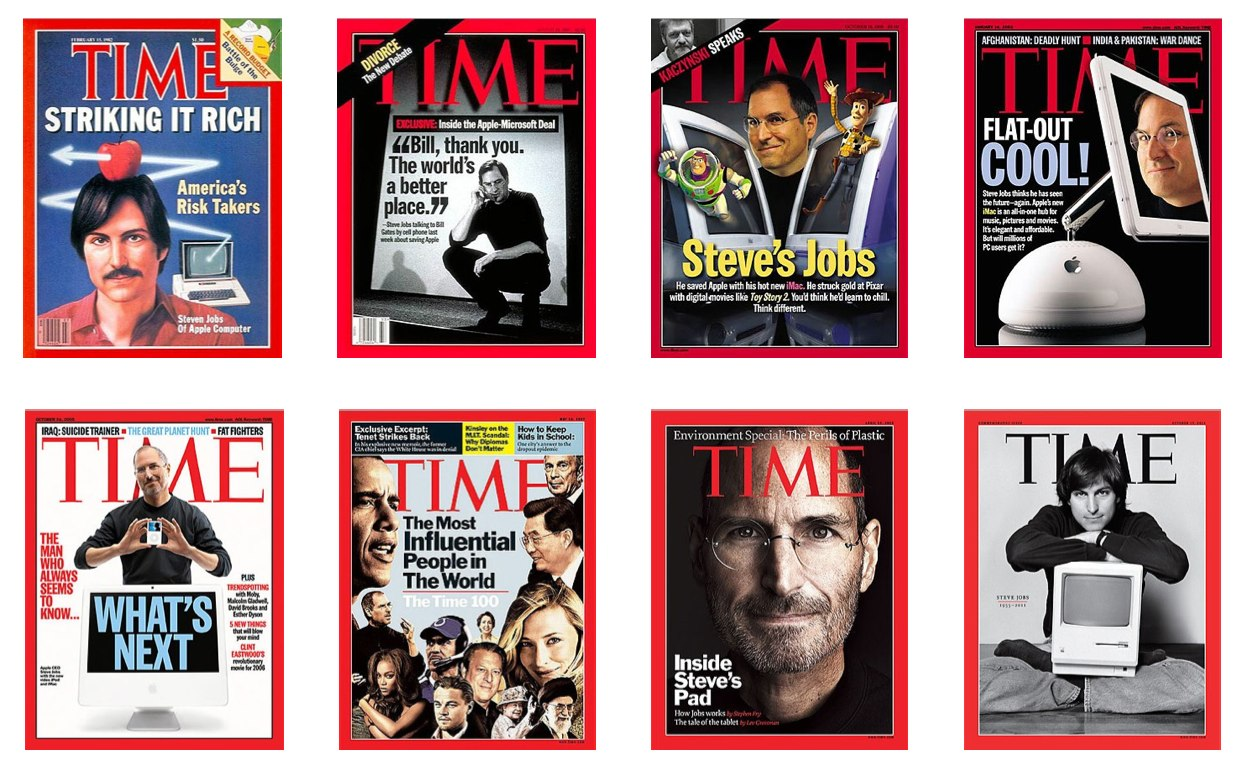
\includegraphics{./images/ch1/time.jpg}}
% 		\resizebox{!}{3cm}{\includegraphics{./images/ch1/Jobs_time_covers/jobs_covers_01.jpg}}\quad
% 		\resizebox{!}{3cm}{\includegraphics{./images/ch1/jobs_time_covers/jobs_covers_02.jpg}}\quad
% 		\resizebox{!}{3cm}{\includegraphics{./images/ch1/jobs_time_covers/jobs_covers_03.jpg}}\quad
% 		\resizebox{!}{3cm}{\includegraphics{./images/ch1/jobs_time_covers/jobs_covers_04.jpg}}
% 		\bigskip
%
% 		\resizebox{!}{3cm}{\includegraphics{./images/ch1/jobs_time_covers/jobs_covers_05.jpg}}\quad
% 		\resizebox{!}{3cm}{\includegraphics{./images/ch1/jobs_time_covers/jobs_covers_06.jpg}}\quad
% 		\resizebox{!}{3cm}{\includegraphics{./images/ch1/jobs_time_covers/jobs_covers_07.jpg}}\quad
% 		\resizebox{!}{3cm}{\includegraphics{./images/ch1/jobs_time_covers/jobs_covers_08.jpg}}
	\end{center}
\end{frame}

\begin{frame}
	\linespread{1.5}
	\begin{columns}
		\column{.42\textwidth}
			\begin{center}
				{
% 				\fontspec{Myriad Pro}
				\bf\Large Stay hungry,\\[5pt]
				stay foolish.
				}
			\end{center}
		\column{.58\textwidth}
			\begin{center}
				\resizebox{7cm}{!}{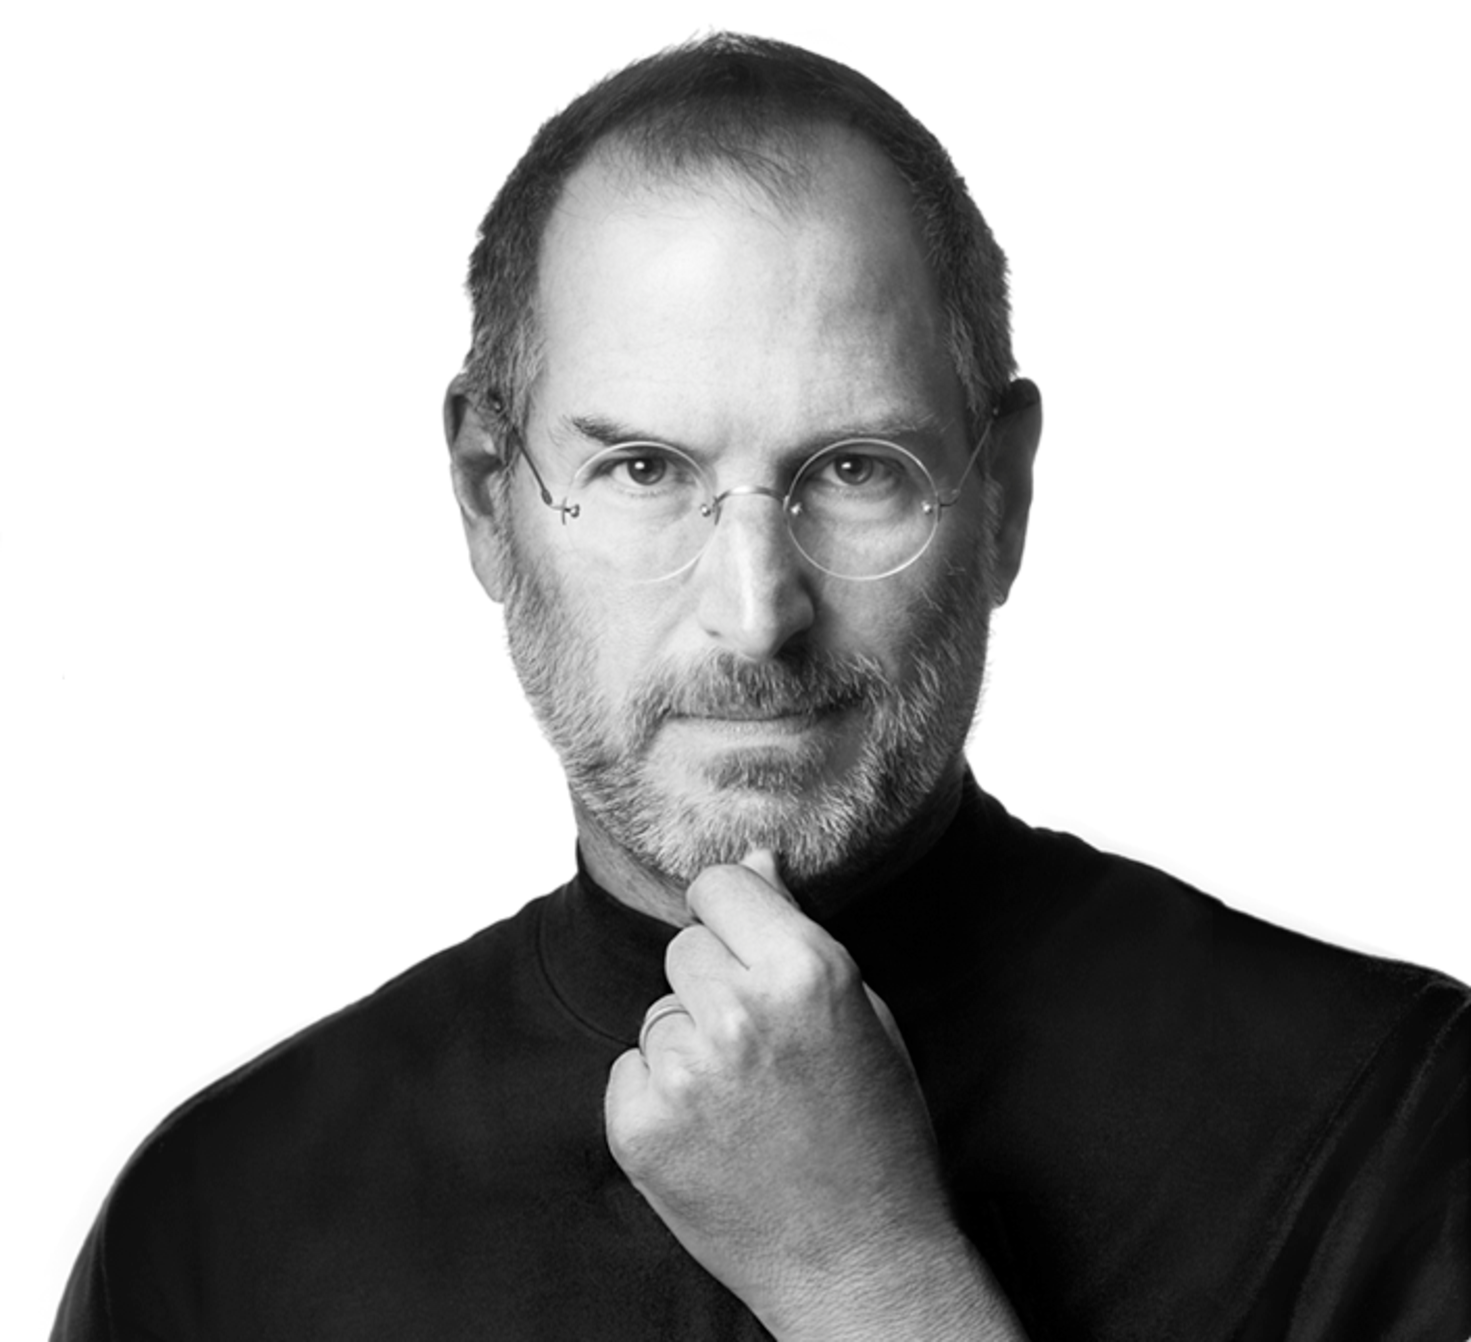
\includegraphics{./images/ch1/t_hero.pdf}}
			\end{center}
	\end{columns}
\end{frame}

\begin{frame}[<+->]{《给未来的你》}
	\linespread{1.4}\pause 
	\begin{enumerate}
	  \item {\bf 寻找兴趣和天赋,避免成为迷茫、困惑的人}
	  \begin{itemize}
	    \item 弄清楚自己想要成为一个什么样的人,特别要知道,自己的兴趣在哪里,天赋在哪里
	    \item \alert{多尝试}
	  \end{itemize}
	  \item {\bf 学会学习和思考,避免成为应试机器}
	  \begin{itemize}
	    \item 自学能力\pause ——\alert{“为什么”}\pause 
	    \item 从理论到实践的能力\pause ——\alert{“有什么用”}\pause 
	    \item 批判式思维的能力\pause ——\alert{“为什么不”}
	  \end{itemize}
	\end{enumerate}
\end{frame}

\begin{frame}[<+->]{《给未来的你》}
	\linespread{1.4}
	\begin{enumerate}
	  \addtocounter{enumi}{2}
	  \item {\bf 培养情商,避免成为孤独、被动的人}
	  \begin{itemize}
	    \item 培养\alert{友情}
	    \item 培养自己的表达能力——\alert{口才}
	    \item 多争取\alert{实习、实践}的机会
	    \item 积极主动,不畏惧失败
	  \end{itemize}
	  \item {\bf 脚踏实地,避免成为浮躁、贪婪的人}
	  \begin{itemize}
	    \item 不要将侥幸致富作为自己的动力
	    \item 注重\alert{诚信}
	    \item \alert{“求知若饥,虚心若愚”}
	  \end{itemize}
	\end{enumerate}
\end{frame}


% \begin{frame}[empty]
% 	\linespread{1.5}
% % 	\newcommand{\chuhao}{\fontsize{72pt}{\baselineskip}\selectfont}
% 	\begin{center}{\ba
% 	{\Huge Welcome, Freshman!!!
% 	}}
% 	\end{center}
% \end{frame}
